\documentclass{article}

\usepackage{graphicx}
\usepackage{hyperref}
\usepackage{float}
\usepackage[backend=biber,style=apa]{biblatex}

\addbibresource{sources.bib}

\title{Roadmap to my future in IT}
\author{Mikołaj Kubś}
\date{\today}

\begin{document}

\maketitle

\section{Introduction}
This document outlines global IT trends for the coming years and a personalized roadmap, partially revised based on the former.

\section{Global trends in IT}
The IT industry is evolving rapidly, driven by technological innovation which shows no signs of slowing down, only pressing the acceleration pedal more and more. Below are some of the key trends over the next five years:

\subsection{Artificial Intelligence and Machine Learning}
\begin{itemize}
    \item \textbf{Generative AI:} the rise of tools like GPT and their application in all industries. LLM's will stand the test of time, whether they can become AGI/ASI (both highly likely in my opinion) or not. But now that this opportunity seems to be more possible than ever, every tech company is trying to rush to develop a machine smarter than a human. An AI general enough to specialize in many environments/technologies etc. would bring unimaginable profits to the company that develops it first.
    \item \textbf{AI ethics:} enhancing transparency in AI models. In case of mass unemployment resulting from smarter than human machines, some anti-AI laws or movements may start to exist. Possible UBI (Universal Basic Income) implementations.
    \item \textbf{AI in gaming:} procedural content generation and dynamic NPC behavior. Easier/automatic creation of meshes and sprites. There may be an anti-AI movement in the gaming community, as some people may prefer the old ways of creating games (there are already some signs of this, but mainly because AI art is still easily recognizable).
\end{itemize}

\subsection{Game development trends}
\begin{itemize}
    \item \textbf{AR/VR and XR:} we'll see if this path attracts more attention. There are already some great VR games, but that hobby is still far from the mainstream and may remain so for a long time. AR is more likely to become mainstream, but it's still hard to predict. In the farther future, AI generated virtual worlds may attract attention.
    \item \textbf{AI - driven game mechanics:} smarter NPCs and adaptive gameplay. Maybe automatically generated and adaptive quests.
    \item \textbf{Aggressive game monetization} games are becoming more and more ambitious, but the companies which monetize their games most aggressively are the ones that are most successful. This trend is likely to continue, as there are some "whales" prone to spending a lot of money on virtual items.
    \item \textbf{Changing games scope} games are becoming so big, that some gamers start to feel overwhelmed. It is possible that in the future, shorter games for adults with limited time will become more popular. After all, people tend to have less free time for leisure as they age, but more money to spend.
\end{itemize}

\subsection{Cybersecurity}
\begin{itemize}
    \item \textbf{AI security:} Protecting against adversarial attacks on AI models. Protection against AI agents autonomously creating buggy code. AI agents may be used to create malware, which could be harder to detect than the one created by humans.
    \item \textbf{Zero trust security:} the rise of zero trust security models. It's possible that in the future, almost all software will be open-source, as it's the only way to be sure that it's secure.
\end{itemize}

\subsection{Technologies of the future}
\begin{itemize}
    \item \textbf{Quantum computing:} the potential to revolutionize computing power. Quantum computing is still in its infancy, but it has the potential to revolutionize the industry. It is possible that quantum computers will be used to create AGI/ASI.
    \item \textbf{5G and beyond:} enabling faster and more connected devices. 5G is already here, but it's still not available everywhere. 6G is already being researched, and it's possible that it will be available in the next 10 years.
    \item \textbf{Space exploration:} the rise of commercial space agencies. The issue with space exploration is that aside putting satellites on Earth's orbit, there is not much more profit to be made. But if we find a way to mine asteroids, that could change and end any shortage of rare metals on Earth.
    \item \textbf{Robotics:} it's extremely likely that autonomous vehicles will take over. It's also possible that robots will start to replace humans in many jobs, but it's hard to predict how fast this will happen. Ironically, it's very possible that intellectual jobs will be easier to automate than many \textit{simple} manual ones. As war in Ukraine progresses, it's clear that drones and other autonomous weapons will be developed more and more.
\end{itemize}

\section{Personal Roadmap}
I have some doubts about my career, and I'm not sure if I am more interested in pursuing a game developer career, or a web developer career (like .NET). Or if automatization using Python (probably with use of AI APIs) is a good career choice (I have a bit of professional experience in that). For now, I'm still sticking with a game developer career, as it's my passion and I have a lot of experience (some professional, mostly personal). As shown in the roadmap from \textcite{game-developer-roadmap}, I have outlined my personal goals and aspirations in the IT industry.

\begin{figure}[H]
    \centering
    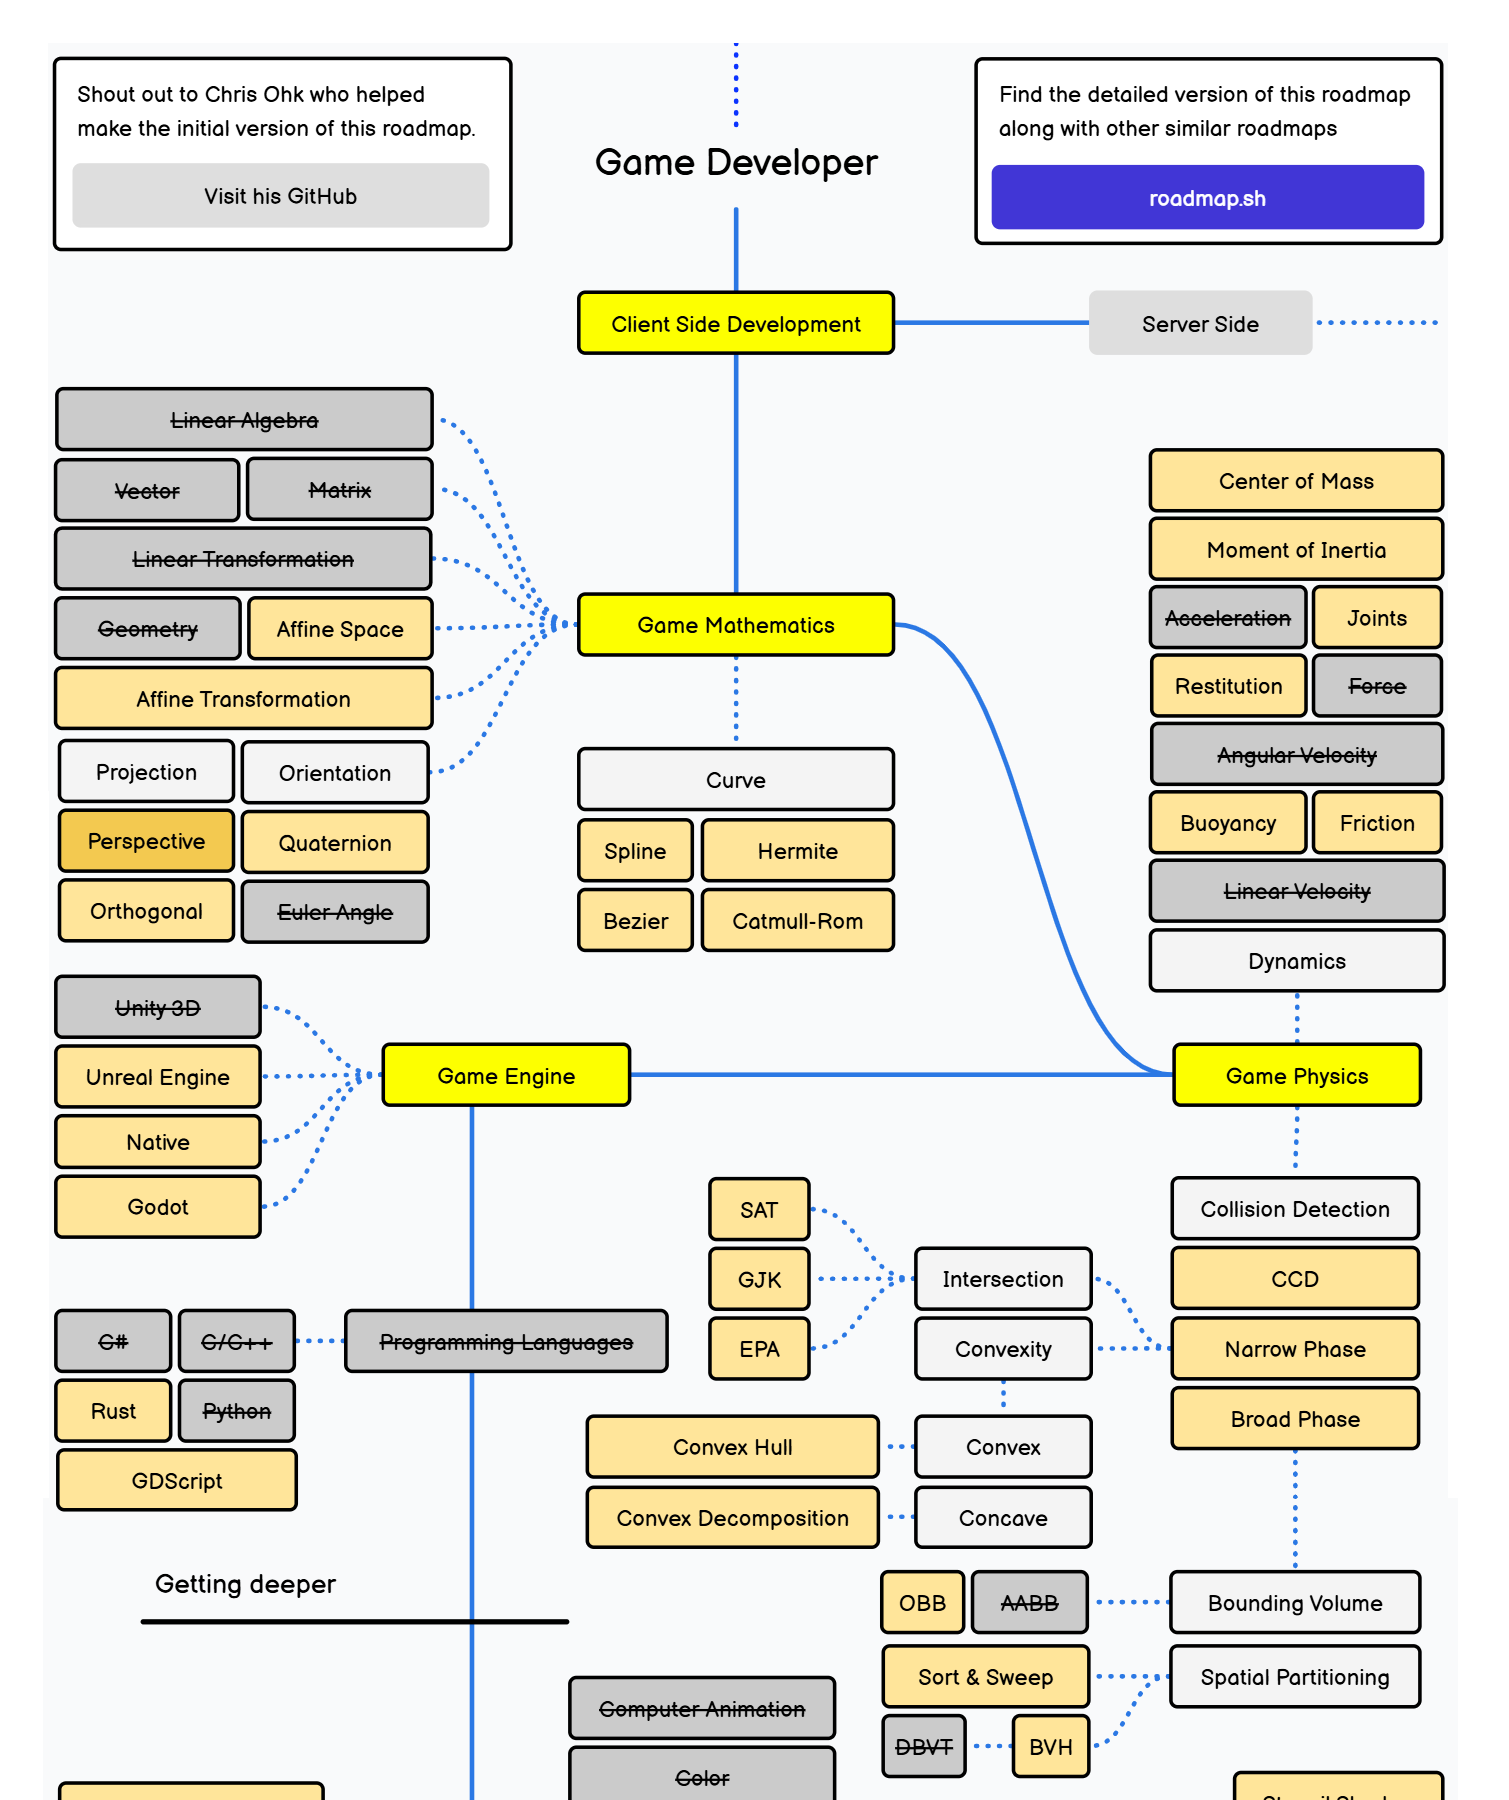
\includegraphics[width=\textwidth]{images/roadmap.png}
    \caption{Roadmap to my future in IT}
    \label{fig:roadmap}
\end{figure}

\begin{figure}[H]
    \centering
    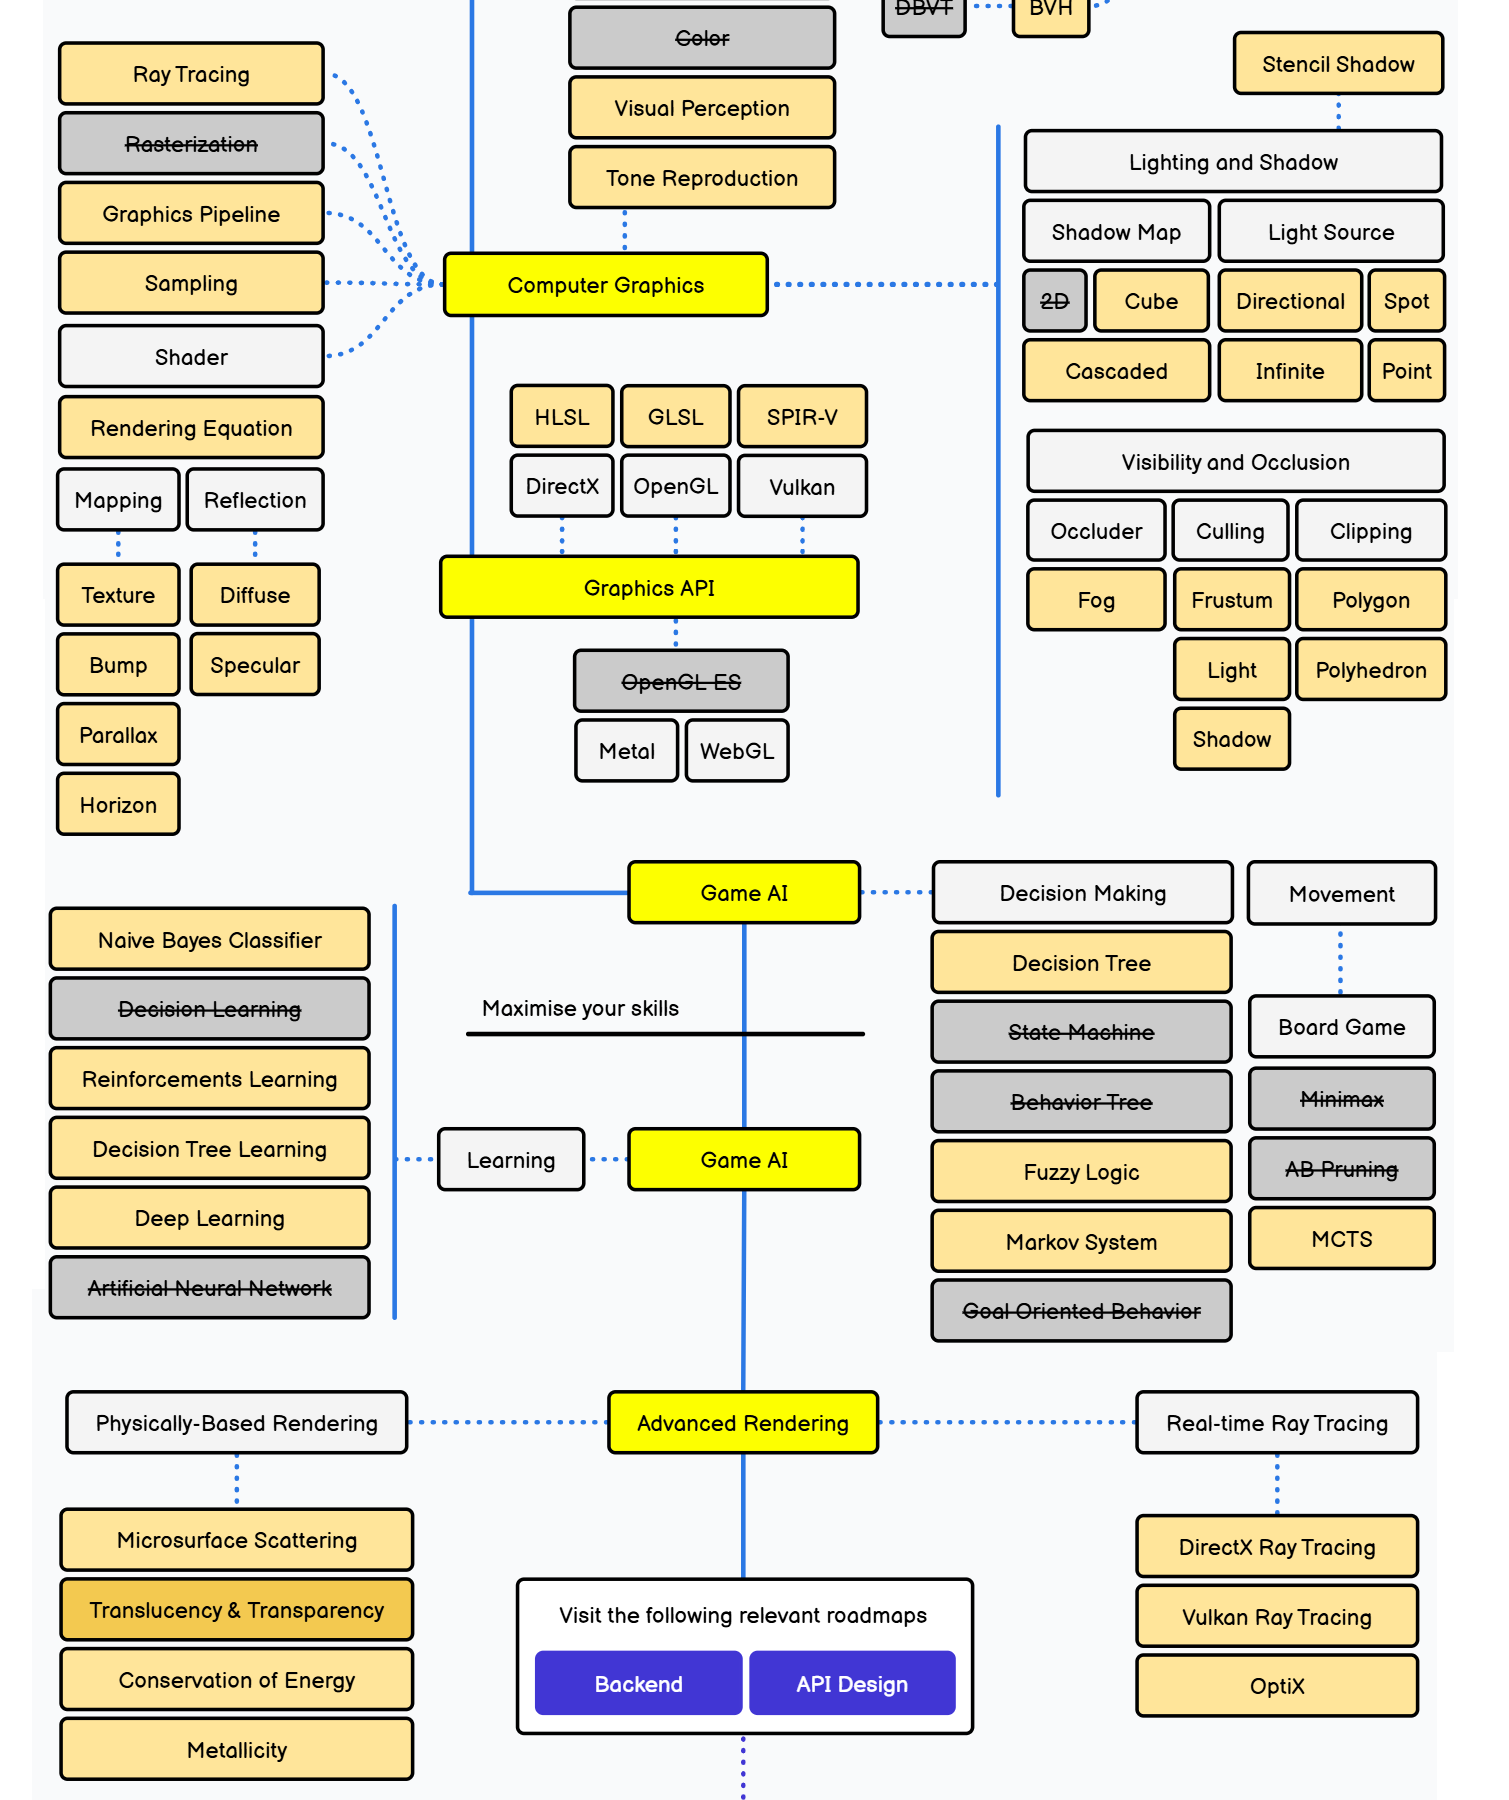
\includegraphics[width=\textwidth]{images/roadmap_2.png}
    \caption{Roadmap to my future in IT: part II}
    \label{fig:roadmap2}
\end{figure}

Looking at this roadmap, it's clear that I still don't know a lot. While I don't think it would be a good idea to strictly learn what I'm missing without applying it, I think creating games out of my comfort zone (AI agents simulations) would be good for my game developer career.

\subsection{2025-2026}
\begin{itemize}
    \item \textbf{AI in game development:} create AI agents using a neural network.
    \item \textbf{Backend skills:} create a game with a backend server using Django and MongoDB.
    \item \textbf{Networking and other engines:} create a multiplayer game in \\Godot/Unreal Engine.
\end{itemize}

\subsection{2027--2028}
\begin{itemize}
    \item \textbf{Game projects:} develop a game featuring procedural content generation.
    \item \textbf{Math in game development:} learn how rendering/shadows/collisions are calculated. Create a very simple game engine in a lower-level language (like C++, not Assembly).
\end{itemize}

\subsection{2029--onwards}
\begin{itemize}
    \item \textbf{Entrepreneurship:} try, with a group of friends, to create a game studio.
\end{itemize}

\subsection{Stop doing}
\begin{itemize}
    \item \textbf{Learning Unity:} I have already learned a lot about Unity, and I think it's time to move on to other engines. They may be less trustworthy, as they may try to aggressively monetize this game engine.
    \item \textbf{Not thinking about a project's architecture:} all my games lack an architecture, and for my AI agents I needed to do a lot of refactoring to make adding new behaviours simpler. It's time to apply more design patterns in practice.
    \item \textbf{Not using network}: I have never created a multiplayer game, and I think it's time to learn how to do it. Or at least how to create a game with a backend server.
\end{itemize}

\section{Conclusion}
It's tough to base my career goals on global trends, as it's very possible that the IT world will change a lot in the coming years and decades. It's possible that an AI may become a better game programmer than me. While that's quite sad, games are a huge project. Maybe with using AI and increasing productivity, truly impressive projects could be created by smaller groups of people. It's also entirely possible that the law of diminishing returns may apply to AI in general, and we are far from true AGI. Anyway, I'm excited for the future, and my part in it.

\printbibliography

\end{document}
